
%\VignetteIndexEntry{Cardinal: Tools for mass spectrometry imaging}
%\VignetteKeyword{Infrastructure, Bioinformatics, Proteomics, MassSpectrometry, Clustering, Classification}

\documentclass[a4paper]{article}

\RequirePackage{/Library/Frameworks/R.framework/Versions/3.1/Resources/library/BiocStyle/sty/Bioconductor}

\AtBeginDocument{\bibliographystyle{/Library/Frameworks/R.framework/Versions/3.1/Resources/library/BiocStyle/sty/unsrturl}}
\title{Cardinal: Analytic tools for mass spectrometry imaging}

\author{Kyle D. Bemis}

\usepackage{Sweave}
\begin{document}
\Sconcordance{concordance:Cardinal-demo.tex:Cardinal-demo.Rnw:%
1 5 1 1 2 1 0 1 2 5 1 1 0 8 1 1 7 4 1 1 6 8 0 2 2 4 0 1 2 2 1 %
1 -4 1 8 3 1 1 2 1 0 1 2 4 0 2 2 4 0 2 2 1 0 2 1 3 0 1 2 11 1 %
1 2 1 0 2 1 3 0 1 2 4 1 1 2 1 0 2 1 3 0 1 2 23 1 1 6 8 0 2 2 %
4 0 1 2 2 1 1 -4 1 8 3 1 1 2 1 0 1 2 4 0 2 2 4 0 2 2 1 0 2 1 %
3 0 1 2 4 1 1 2 4 0 1 3 4 0 1 2 3 1 1 -8 1 12 1 -9 1 13 4 1 1 %
2 4 0 1 3 4 0 1 2 3 1 1 -8 1 12 1 -9 1 13 4 1 1 2 4 0 1 2 2 1 %
1 -4 1 8 6 1 1 2 4 0 1 3 4 0 1 2 3 1 1 -8 1 12 1 -9 1 13 4 1 %
1 2 4 0 1 3 4 0 1 2 3 1 1 -8 1 12 1 -9 1 13 4 1 1 2 4 0 1 2 2 %
1 1 -4 1 8 21 1 1 2 4 0 1 3 4 0 1 2 2 1 1 -7 1 11 6 1 1 2 4 0 %
1 3 4 0 1 3 4 0 1 2 3 1 1 -11 1 15 1 -12 1 16 7 1 1 2 4 0 1 3 %
4 0 1 2 2 1 1 -7 1 11 6 1 1 2 4 0 1 3 4 0 1 3 4 0 1 2 3 1 1 %
-11 1 15 1 -12 1 16 7 1 1 2 4 0 1 3 4 0 1 2 2 1 1 -7 1 11 6 1 %
1 2 4 0 1 3 4 0 1 3 4 0 1 2 3 1 1 -11 1 15 1 -12 1 16 17 1 1 %
6 8 0 2 2 4 0 1 2 2 1 1 -4 1 8 3 1 1 2 1 0 1 2 4 0 2 2 4 0 2 %
2 1 0 2 1 3 0 1 2 5 1 1 2 1 0 1 1 37 0 2 2 37 0 2 2 1 0 1 1 3 %
0 1 3 1 0 1 1 3 0 1 2 3 1 1 -9 1 13 1 -9 1 13 8 1 1 2 1 0 1 1 %
26 0 2 2 4 0 1 3 4 0 1 2 3 1 1 -8 1 12 1 -9 1 13 17 1 1 2 11 %
0 1 2 1 1}


\maketitle

\tableofcontents

\section{Introduction}

This will be a brief walkthrough of some of the basic functionality of Cardinal.

\section{Setup}

For the following examples, we will use a simulated dataset. The image is a cardinal with red and black feathers, where the colors represent different regions of the image. The mass spectra will have two peaks to indicate the two regions. We use \Robject{generateImage} to generate the dataset from an integer matrix where $0$ represents black regions of the image and $1$ represents the red regions of the image.
\begin{Schunk}
\begin{Sinput}
> data <- matrix(c(NA, NA, 1, 1, NA, NA, NA, NA, NA, NA, 1, 1, NA, NA, 
+  NA, NA, NA, NA, NA, 0, 1, 1, NA, NA, NA, NA, NA, 1, 0, 0, 1, 
+  1, NA, NA, NA, NA, NA, 0, 1, 1, 1, 1, NA, NA, NA, NA, 0, 1, 1, 
+  1, 1, 1, NA, NA, NA, NA, 1, 1, 1, 1, 1, 1, 1, NA, NA, NA, 1, 
+  1, NA, NA, NA, NA, NA, NA, 1, 1, NA, NA, NA, NA, NA), nrow=9, ncol=9)
\end{Sinput}
\end{Schunk}
We can plot the ground truth image directly.
\begin{Schunk}
\begin{Sinput}
> image(data[,ncol(data):1], col=c("black", "red"))
\end{Sinput}
\end{Schunk}
\setkeys{Gin}{width=0.4\textwidth}
\begin{figure}
\begin{center}
\includegraphics{Cardinal-demo-005}
\caption{\small Ground truth image used to generate the simulated dataset.}
\end{center}
\end{figure}
Now we generate the data as if from a mass spectrometry imaging experiment with peaks at $m/z$ 3000 (higher intensity in black pixels) and $m/z$ 4000 (higher intensity in red pixels).
\begin{Schunk}
\begin{Sinput}
> set.seed(1)
> msset <- generateImage(data, range=c(1000,5000), centers=c(3000,4000), resolution=100,
+ 	step=3.3, as="MSImageSet")
\end{Sinput}
\end{Schunk}
We need to mark which pixels are black and which are red.
\begin{Schunk}
\begin{Sinput}
> pData(msset)$pg <- factor(data[is.finite(data)], labels=c("black", "red"))
\end{Sinput}
\end{Schunk}
Then we need to mark which features (which regions of the mass spectrum) belong to the peaks associated with ``black'' or ``red'' pixels; the rest of the spectrum is marked as background noise (\texttt{bg}).
\begin{Schunk}
\begin{Sinput}
> fData(msset)$fg <- factor(rep("bg", nrow(fData(msset))), levels=c("bg", "black", "red"))
> fData(msset)$fg[2950 < fData(msset)$mz & fData(msset)$mz < 3050] <- "black"
> fData(msset)$fg[3950 < fData(msset)$mz & fData(msset)$mz < 4050] <- "red"
\end{Sinput}
\end{Schunk}
Now we can experiment with different ways of working with a mass spectrometry imaging dataset in \Rpackage{Cardinal}.



\section{Input/Output}
\subsection{Input}
\Rpackage{Cardinal} can read two of the most common data exchange formats in imaging mass spectrometry: Analyze 7.5 and imzML.

\subsubsection{Analyze 7.5}

Originally designed for MRI use, Analyze 7.5 is one of the oldest and most common formats still used for exchange of mass spectrometry imaging data.

\begin{Schunk}
\begin{Sinput}
> name <- "Bierbaum_demo_"
> folder <- "/Users/kuwisdelu/Documents/Datasets/DESI-Imaging/Bierbaum_demo_"
> x1 <- readAnalyze(name=name, folder=folder)
\end{Sinput}
\end{Schunk}

\subsubsection{imzML}

A newly-developed format specifically designed for interchange of mass spectrometry imaging datasets, imzML is an open XML-based format to which many other formats can be converted.

\begin{Schunk}
\begin{Sinput}
> name <- "S042_Continuous"
> folder <- "/Users/kuwisdelu/Documents/Purdue/Research/Imaging/Data and Code/imzML/s042_continuous/"
> x2 <- readImzML(name=name, folder=folder)
\end{Sinput}
\end{Schunk}

\subsection{Output}

\subsubsection{RData files}

Any R object including \Robject{MSImageSet} datasets can be exported and saved as an \textbf{RData} file using \verb|save| and reimported using \verb|load|.


\section{Subsetting and Inspecting Data}





\section{Plotting}
One of the most important parts of working with mass spectrometry imaging datasets is visualization of the data by examining the ion images and mass spectra. \Rpackage{Cardinal} provides powerful functionality for plotting both ion images, mass spectra, as well as other representations of imaging data.

\subsection{Formula interface}

The plotting facilities of \Rpackage{Cardinal} are based on the powerful formula interface used by the \Robject{lattice} graphics package.

\subsection{Plotting using \Rpackage{Cardinal}}

For the following examples, we will use a simulated dataset. The image is a cardinal with red and black feathers, where the colors represent different regions of the image. The mass spectra will have two peaks to indicate the two regions. We use \Robject{generateImage} to generate the dataset from an integer matrix where $0$ represents black regions of the image and $1$ represents the red regions of the image.
\begin{Schunk}
\begin{Sinput}
> data <- matrix(c(NA, NA, 1, 1, NA, NA, NA, NA, NA, NA, 1, 1, NA, NA, 
+  NA, NA, NA, NA, NA, 0, 1, 1, NA, NA, NA, NA, NA, 1, 0, 0, 1, 
+  1, NA, NA, NA, NA, NA, 0, 1, 1, 1, 1, NA, NA, NA, NA, 0, 1, 1, 
+  1, 1, 1, NA, NA, NA, NA, 1, 1, 1, 1, 1, 1, 1, NA, NA, NA, 1, 
+  1, NA, NA, NA, NA, NA, NA, 1, 1, NA, NA, NA, NA, NA), nrow=9, ncol=9)
\end{Sinput}
\end{Schunk}
We can plot the ground truth image directly.
\begin{Schunk}
\begin{Sinput}
> image(data[,ncol(data):1], col=c("black", "red"))
\end{Sinput}
\end{Schunk}
\setkeys{Gin}{width=0.4\textwidth}
\begin{figure}
\begin{center}
\includegraphics{Cardinal-demo-013}
\caption{\small Ground truth image used to generate the simulated dataset.}
\end{center}
\end{figure}
Now we generate the data as if from a mass spectrometry imaging experiment with peaks at $m/z$ 3000 (higher intensity in black pixels) and $m/z$ 4000 (higher intensity in red pixels).
\begin{Schunk}
\begin{Sinput}
> set.seed(1)
> msset <- generateImage(data, range=c(1000,5000), centers=c(3000,4000), resolution=100,
+   step=3.3, as="MSImageSet")
\end{Sinput}
\end{Schunk}
We need to mark which pixels are black and which are red.
\begin{Schunk}
\begin{Sinput}
> pData(msset)$pg <- factor(data[is.finite(data)], labels=c("black", "red"))
\end{Sinput}
\end{Schunk}
Then we need to mark which features (which regions of the mass spectrum) belong to the peaks associated with ``black'' or ``red'' pixels; the rest of the spectrum is marked as background noise (\texttt{bg}).
\begin{Schunk}
\begin{Sinput}
> fData(msset)$fg <- factor(rep("bg", nrow(fData(msset))), levels=c("bg", "black", "red"))
> fData(msset)$fg[2950 < fData(msset)$mz & fData(msset)$mz < 3050] <- "black"
> fData(msset)$fg[3950 < fData(msset)$mz & fData(msset)$mz < 4050] <- "red"
\end{Sinput}
\end{Schunk}
Now we can experiment with different ways of plotting an imaging dataset.

\subsubsection{Plotting mass spectra}

The \verb|plot| method is used to plot mass spectra. The \Robject{pixel} argument is used to specify the pixel to use to plot the mass spectrum. If no conditioning is desired, the formula does not need to be specified explicitly.
\begin{Schunk}
\begin{Sinput}
> plot(msset, pixel=1)
\end{Sinput}
\end{Schunk}
\begin{Schunk}
\begin{Sinput}
> plot(msset, ~ mz, pixel=1)
\end{Sinput}
\end{Schunk}
\setkeys{Gin}{width=0.4\textwidth}
\begin{figure}
\begin{center}
\begin{tabular}{cc}
\includegraphics{Cardinal-demo-019}
&
\includegraphics{Cardinal-demo-020}
\end{tabular}
\caption{\small A simple mass spectrum plot. Both forms produce the same plot.}
\end{center}
\end{figure}
Specifying multiple pixels will apply a function, specified by \Robject{fun}, over those pixels. This can be used to create a plot of the mean spectrum (the default behavior). Below we obtain the mean spectrum of the red pixels, and the max spectrum of the black pixels.
\begin{Schunk}
\begin{Sinput}
> plot(msset, pixel=pData(msset)$pg=="red", fun=median, main="Median of red pixels")
\end{Sinput}
\end{Schunk}
\begin{Schunk}
\begin{Sinput}
> plot(msset, pixel=pData(msset)$pg=="black", fun=max, main="Max of black pixels")
\end{Sinput}
\end{Schunk}
\begin{figure}
\setkeys{Gin}{width=0.4\textwidth}
\begin{center}
\begin{tabular}{cc}
\includegraphics{Cardinal-demo-023}
&
\includegraphics{Cardinal-demo-024}
\end{tabular}
\caption{\small Applying a function over pixels to plot a median and max spectrum.}
\end{center}
\end{figure}
Using the \Robject{lattice} graphics option allows for more complex plots to be made. Conditioning on variables in the \Robject{formula} argument allows direct comparison between regions of the image or mass spectrum. For example, by conditioning on the variable \verb|pData(msset)$pg| which specifies the color of the pixels, we can obtain mean spectra for each type of pixel in a single step; notice that the \verb|plot| method knows where to find the \Robject{pg} variable, because it is contained in \Robject{msset}. Likewise, we use the \Robject{fg} variable (which we used to mark notable $m/z$-values) with the argument \Robject{groups} to distinguish different regions of the mass spectrum with different colors.
\begin{Schunk}
\begin{Sinput}
> print(plot(msset, ~ mz | pg, pixel=1:ncol(msset), groups=fg, lattice=TRUE, col=c("blue", "black", "red")))
\end{Sinput}
\end{Schunk}
\begin{figure}
\setkeys{Gin}{width=0.8\textwidth}
\begin{center}
\includegraphics{Cardinal-demo-026}
\caption{\small A plot conditioning on variables using \Robject{lattice} graphics.}
\end{center}
\end{figure}

\subsubsection{Plotting ion images}

The \verb|image| method is used to plot images. The \Robject{feature} argument is used to specify the feature to use to create the image. For a mass spectrometry imaging dataset, the features are the $m/z$-values corresponding to single-ion images. As before, if no conditioning is desired, the formula does not need to be specified explicitly.
\begin{Schunk}
\begin{Sinput}
> image(msset, feature=1, col.regions=gradient.colors(100, "red", "black"))
\end{Sinput}
\end{Schunk}
\begin{Schunk}
\begin{Sinput}
> image(msset, ~ x * y, feature=1, col.regions=gradient.colors(100, "red", "black"))
\end{Sinput}
\end{Schunk}
\begin{figure}
\setkeys{Gin}{width=0.4\textwidth}
\begin{center}
\begin{tabular}{cc}
\includegraphics{Cardinal-demo-029}
&
\includegraphics{Cardinal-demo-030}
\end{tabular}
\caption{\small A simple single-ion image. Both forms produce the same plot.}
\end{center}
\end{figure}
Like with the \verb|plot| method, the \verb|image| method can apply functions over features ($m/z$-values) when multiple features are specified. By default, \verb|mean| is used to average the images over the features. In the following example, we specify two plots, first using the features from the peak that has a higher intensity associated with black pixels, and then using the features from the peak that has a higher intensity associated with red pixels.
\begin{Schunk}
\begin{Sinput}
> image(msset, feature=fData(msset)$fg=="black", col.regions=alpha.colors(100, "black"))
\end{Sinput}
\end{Schunk}
\begin{Schunk}
\begin{Sinput}
> image(msset, feature=fData(msset)$fg=="red", col.regions=alpha.colors(100, "red"))
\end{Sinput}
\end{Schunk}
\begin{figure}
\setkeys{Gin}{width=0.4\textwidth}
\begin{center}
\begin{tabular}{cc}
\includegraphics{Cardinal-demo-033}
&
\includegraphics{Cardinal-demo-034}
\end{tabular}
\caption{\small Averaging over different sets of mass features.}
\end{center}
\end{figure}
Using a \Robject{lattice}-style formula, we can condition on other variables with \verb|image| too. Here we use all of the features, but condition on which part of the mass spectrum those features come from using the variable \verb|fData(msset)$fg|. Again, since \verb|image| knows to look in \Robject{msset}, we only need to specify the variable as \Robject{fg}.
\begin{Schunk}
\begin{Sinput}
> print(image(msset, ~ x * y | fg, feature=1:nrow(msset), col.regions=intensity.colors(100), lattice=TRUE))
\end{Sinput}
\end{Schunk}
\begin{figure}
\setkeys{Gin}{width=0.8\textwidth}
\begin{center}
\includegraphics{Cardinal-demo-036}
\caption{\small Images conditioning on variables using \Robject{lattice} graphics.}
\end{center}
\end{figure}





\section{Pre-processing}

\setkeys{Gin}{width=\textwidth}
\begin{figure}
\begin{center}
\includegraphics{preprocessingRoughDraft.pdf}
\caption{\small Preprocessing steps}
\end{center}
\end{figure}


\subsection{Normalization}

Normalization is perhaps the most important pre-processing step before any kind of analysis should be performed on biological datasets, and mass spectrometry imaging experiments are no different in this regard. \Rpackage{Cardinal} provides normalization to total ion current (TIC). In the first command below, we only perform the normalization on the first pixel in order to show a plot of the processing results. In the second, we perform normalization on the whole dataset.
\begin{Schunk}
\begin{Sinput}
> temp <- normalize(msset, pixel=1, method="tic", plot=TRUE)
\end{Sinput}
\end{Schunk}
\begin{Schunk}
\begin{Sinput}
> msset2 <- normalize(msset, method="tic")
\end{Sinput}
\end{Schunk}
\setkeys{Gin}{width=0.4\textwidth}
\begin{figure}
\begin{center}
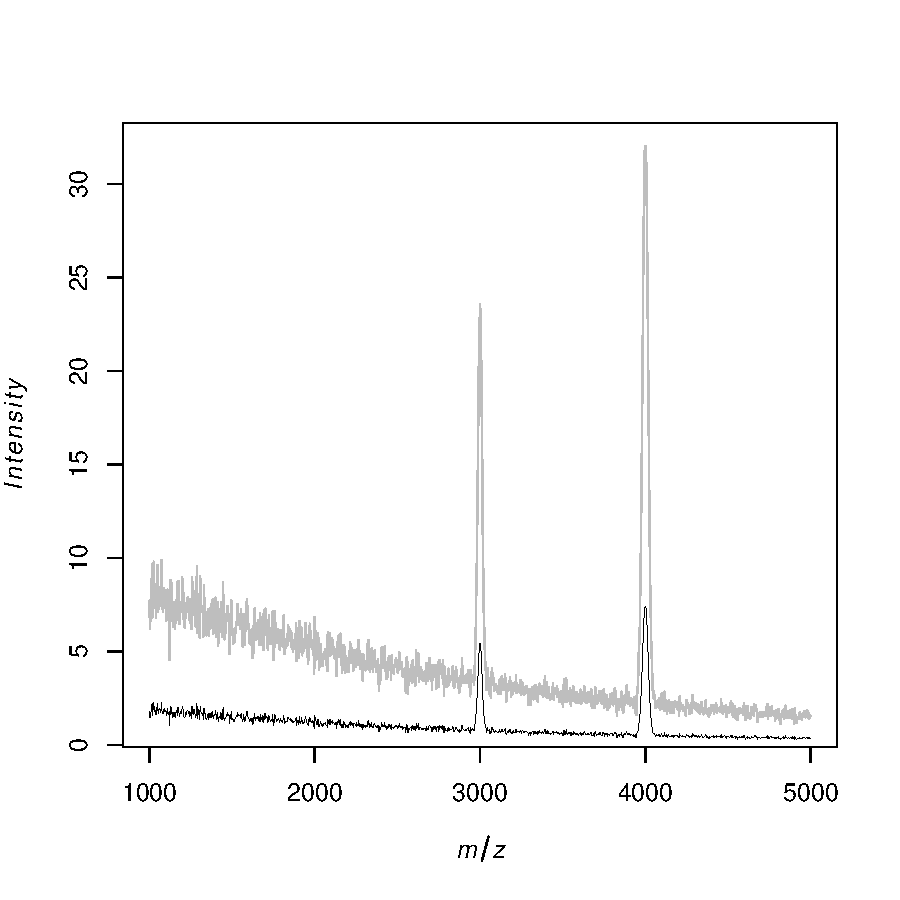
\includegraphics{Cardinal-demo-039}
\caption{\small Total ion current (TIC) normalization.}
\end{center}
\end{figure}

\subsection{Smoothing}

Smoothing the mass spectra is useful for removing noise, which can improve detection of peaks. \Rpackage{Cardinal} provides several common methods for smoothing mass spectra, including Gaussian kernel smoothing, Savitsky-Golay smoothing, and a simple moving average filter.
\begin{Schunk}
\begin{Sinput}
> temp <- smoothSignal(msset2, pixel=1, method="gaussian", window=9, plot=TRUE)
\end{Sinput}
\end{Schunk}
\begin{Schunk}
\begin{Sinput}
> temp <- smoothSignal(msset2, pixel=1, method="sgolay", window=15, plot=TRUE)
\end{Sinput}
\end{Schunk}
\begin{Schunk}
\begin{Sinput}
> msset3 <- smoothSignal(msset2, method="gaussian", window=9)
\end{Sinput}
\end{Schunk}
\begin{figure}
\setkeys{Gin}{width=0.4\textwidth}
\begin{center}
\begin{tabular}{ccc}
\includegraphics{Cardinal-demo-043}
&
\includegraphics{Cardinal-demo-044}
\end{tabular}
\caption{\small Gaussian smoothing and Savitsky-Golay smoothing.}
\end{center}
\end{figure}

\subsection{Baseline reduction}

Baseline reduction is often necessary for many datasets, and \Rpackage{Cardinal} implements a simple version that interpolates a baseline from local medians or local minima, while attempting to preserve the signal from mass spectral peaks.
\begin{Schunk}
\begin{Sinput}
> temp <- reduceBaseline(msset3, pixel=1, method="median", blocks=50, plot=TRUE)
\end{Sinput}
\end{Schunk}
\begin{Schunk}
\begin{Sinput}
> msset4 <- reduceBaseline(msset3, method="median", blocks=50)
\end{Sinput}
\end{Schunk}
\setkeys{Gin}{width=0.4\textwidth}
\begin{figure}
\begin{center}
\includegraphics{Cardinal-demo-047}
\caption{\small Baseline reduction using interpolation from medians.}
\end{center}
\end{figure}

\subsection{Peak picking}

Peak picking is a common form of data reduction that reduces the signal to relevant data peaks. \Rpackage{Cardinal} implements three varieties based on a user-specified signal-to-noise ratio (SNR). The ``simple'' version interpolates a constant noise pattern, the ``adaptive'' version interpolates an adaptive noise pattern, and ``limpic'' implements the LIMPIC algorithm for peak detection.
\begin{Schunk}
\begin{Sinput}
> temp <- peakPick(msset4, pixel=1, method="adaptive", SNR=3, plot=TRUE)
\end{Sinput}
\end{Schunk}
\begin{Schunk}
\begin{Sinput}
> temp <- peakPick(msset4, pixel=1, method="limpic", SNR=3, plot=TRUE)
\end{Sinput}
\end{Schunk}
\begin{Schunk}
\begin{Sinput}
> msset5 <- peakPick(msset4, method="simple", SNR=3)
\end{Sinput}
\end{Schunk}
\begin{figure}
\setkeys{Gin}{width=0.4\textwidth}
\begin{center}
\begin{tabular}{cc}
\includegraphics{Cardinal-demo-051}
&
\includegraphics{Cardinal-demo-052}
\end{tabular}
\caption{\small Peak picking with adaptive noise and LIMPIC.}
\end{center}
\end{figure}

\subsection{Peak alignment}

Peak alignment is necessary to account for possible inaccuracy in m/z measurements. Peaks can be aligned to a reference list of known m/z values, or to the local maxima in the mean spectrum.
\begin{Schunk}
\begin{Sinput}
> temp <- peakAlign(msset5, pixel=1, method="diff", plot=TRUE)
\end{Sinput}
\end{Schunk}
\begin{Schunk}
\begin{Sinput}
> msset6 <- peakAlign(msset5, method="diff")
\end{Sinput}
\end{Schunk}
\setkeys{Gin}{width=0.4\textwidth}
\begin{figure}
\begin{center}
\includegraphics{Cardinal-demo-055}
\caption{\small Peak alignment to the local maxima of the mean spectrum.}
\end{center}
\end{figure}

\subsection{Data reduction}

Other common forms of data reduction include resampling and binning.
\begin{Schunk}
\begin{Sinput}
> temp <- reduceDimension(msset4, pixel=1, method="bin", width=25, fun=mean, plot=TRUE)
\end{Sinput}
\end{Schunk}
\begin{Schunk}
\begin{Sinput}
> temp <- reduceDimension(msset4, pixel=1, method="resample", step=25, plot=TRUE)
\end{Sinput}
\end{Schunk}
\begin{Schunk}
\begin{Sinput}
> msset7 <- reduceDimension(msset4, method="resample", step=25)
\end{Sinput}
\end{Schunk}
\begin{figure}
\setkeys{Gin}{width=0.4\textwidth}
\begin{center}
\begin{tabular}{cc}
\includegraphics{Cardinal-demo-059}
&
\includegraphics{Cardinal-demo-060}
\end{tabular}
\caption{\small Data reduction via binning and resampling.}
\end{center}
\end{figure}





\section{Analysis}


\section{Advanced Topics}

\subsection{Apply}
The \verb|apply| family of functions are a powerful feature of \R. The \verb|apply| function applies a function over margins of an array, while \verb|sapply| applies a function over every element of a vector-like object. The function \verb|tapply| applies a function over a ``ragged'' array, so that the function is applied over groups of values given by levels of another variable (usually a factor). In \Rpackage{Cardinal}, the methods \verb|pixelApply| and \verb|featureApply| allow \verb|apply|-like functionality that combine traits of each of these, tailored for imaging datasets.

For the following examples, we will use a simulated dataset. The image is a cardinal with red and black feathers, where the colors represent different regions of the image. The mass spectra will have two peaks to indicate the two regions. We use \Robject{generateImage} to generate the dataset from an integer matrix where $0$ represents black regions of the image and $1$ represents the red regions of the image.
\begin{Schunk}
\begin{Sinput}
> data <- matrix(c(NA, NA, 1, 1, NA, NA, NA, NA, NA, NA, 1, 1, NA, NA, 
+  NA, NA, NA, NA, NA, 0, 1, 1, NA, NA, NA, NA, NA, 1, 0, 0, 1, 
+  1, NA, NA, NA, NA, NA, 0, 1, 1, 1, 1, NA, NA, NA, NA, 0, 1, 1, 
+  1, 1, 1, NA, NA, NA, NA, 1, 1, 1, 1, 1, 1, 1, NA, NA, NA, 1, 
+  1, NA, NA, NA, NA, NA, NA, 1, 1, NA, NA, NA, NA, NA), nrow=9, ncol=9)
\end{Sinput}
\end{Schunk}
We can plot the ground truth image directly.
\begin{Schunk}
\begin{Sinput}
> image(data[,ncol(data):1], col=c("black", "red"))
\end{Sinput}
\end{Schunk}
\setkeys{Gin}{width=0.4\textwidth}
\begin{figure}
\begin{center}
\includegraphics{Cardinal-demo-063}
\caption{\small Ground truth image used to generate the simulated dataset.}
\end{center}
\end{figure}
Now we generate the data as if from a mass spectrometry imaging experiment with peaks at $m/z$ 3000 (higher intensity in black pixels) and $m/z$ 4000 (higher intensity in red pixels).
\begin{Schunk}
\begin{Sinput}
> set.seed(1)
> msset <- generateImage(data, range=c(1000,5000), centers=c(3000,4000), resolution=100,
+   step=3.3, as="MSImageSet")
\end{Sinput}
\end{Schunk}
We need to mark which pixels are black and which are red.
\begin{Schunk}
\begin{Sinput}
> pData(msset)$pg <- factor(data[is.finite(data)], labels=c("black", "red"))
\end{Sinput}
\end{Schunk}
Then we need to mark which features (which regions of the mass spectrum) belong to the peaks associated with ``black'' or ``red'' pixels; the rest of the spectrum is marked as background noise (\texttt{bg}).
\begin{Schunk}
\begin{Sinput}
> fData(msset)$fg <- factor(rep("bg", nrow(fData(msset))), levels=c("bg", "black", "red"))
> fData(msset)$fg[2950 < fData(msset)$mz & fData(msset)$mz < 3050] <- "black"
> fData(msset)$fg[3950 < fData(msset)$mz & fData(msset)$mz < 4050] <- "red"
\end{Sinput}
\end{Schunk}
Now we can experiment with different ways of plotting an imaging dataset.

\subsubsection{\Robject{pixelApply}}

The method \verb|pixelApply| allows functions to be applied over all pixels. The function is applied pixel-by-pixel to the feature vectors (mass spectra). Here, we use \verb|pixelApply| to find the pixel-by-pixel mean intensity of different regions of the mass spectrum. We provide \verb|fData(msset)$fg| as a grouping variable, since it indicates different regions of the mass spectrum we expect to be associated with either background noise, or red or black pixels. Since \verb|pixelApply| knows to look in \Robject{msset} for the variable, we only need to provide \Robject{fg} to the argument \Robject{.feature.groups}.

\begin{Schunk}
\begin{Sinput}
> p1 <- pixelApply(msset, mean, .feature.groups=fg)
> p1[,1:30]
\end{Sinput}
\begin{Soutput}
      x = 3, y = 1 x = 4, y = 1 x = 2, y = 2 x = 3, y = 2
bg        3.890303     3.935974     3.852787     3.789505
black     9.635005    10.517746     9.308453    10.440883
red      14.765521    15.123040    14.341188    14.303296
      x = 2, y = 3 x = 3, y = 3 x = 4, y = 3 x = 1, y = 4
bg        4.976931     3.960794     4.028191     4.145899
black    16.728553    10.093288    10.064517     9.532089
red       9.241133    15.285169    15.723496    15.951808
      x = 2, y = 4 x = 3, y = 4 x = 4, y = 4 x = 5, y = 4
bg        4.632393     4.863252     3.813765     4.065992
black    15.457280    16.399439    11.023859    10.385429
red       8.928271     9.437796    14.641915    15.559322
      x = 2, y = 5 x = 3, y = 5 x = 4, y = 5 x = 5, y = 5
bg        4.853165     4.189047     3.613069     4.109948
black    16.177474     9.967317     9.820366    10.696623
red       8.958284    16.241629    13.738381    15.884999
      x = 6, y = 5 x = 2, y = 6 x = 3, y = 6 x = 4, y = 6
bg        4.516140     4.230802     4.146095     4.120097
black     9.599486    13.888708     9.756209     9.680859
red      17.661532     8.354190    16.029427    15.867799
      x = 5, y = 6 x = 6, y = 6 x = 7, y = 6 x = 3, y = 7
bg        4.334037     3.876803     3.702975     4.190092
black     9.174036    10.088559     9.622180    11.097352
red      16.825779    14.652355    13.854740    16.202813
      x = 4, y = 7 x = 5, y = 7 x = 6, y = 7 x = 7, y = 7
bg        3.848391     4.028779     4.018565     3.932754
black     9.506104    10.272061     9.273227    10.025520
red      14.646689    15.464322    15.394325    14.869473
      x = 8, y = 7 x = 9, y = 7
bg        3.855238     4.112314
black     9.227148    10.014673
red      14.623218    15.741579
\end{Soutput}
\end{Schunk}
By comparing side-by-side with the ground truth (which we have stored in the variable \verb|pData(msset)$pg|), we see the result is as we expected. For ``black'' pixels, the mean intensity of features belonging to the ``black''-associated peak ($m/z$ 3000) is higher, while for the ``red'' pixels, the mean intensity of features belonging to the ``red''-associated peak ($m/z$ 4000) is higher.
\begin{Schunk}
\begin{Sinput}
> cbind(pData(msset), t(p1))[1:30,c("pg", "black", "red")]
\end{Sinput}
\begin{Soutput}
                pg     black       red
x = 3, y = 1   red  9.635005 14.765521
x = 4, y = 1   red 10.517746 15.123040
x = 2, y = 2   red  9.308453 14.341188
x = 3, y = 2   red 10.440883 14.303296
x = 2, y = 3 black 16.728553  9.241133
x = 3, y = 3   red 10.093288 15.285169
x = 4, y = 3   red 10.064517 15.723496
x = 1, y = 4   red  9.532089 15.951808
x = 2, y = 4 black 15.457280  8.928271
x = 3, y = 4 black 16.399439  9.437796
x = 4, y = 4   red 11.023859 14.641915
x = 5, y = 4   red 10.385429 15.559322
x = 2, y = 5 black 16.177474  8.958284
x = 3, y = 5   red  9.967317 16.241629
x = 4, y = 5   red  9.820366 13.738381
x = 5, y = 5   red 10.696623 15.884999
x = 6, y = 5   red  9.599486 17.661532
x = 2, y = 6 black 13.888708  8.354190
x = 3, y = 6   red  9.756209 16.029427
x = 4, y = 6   red  9.680859 15.867799
x = 5, y = 6   red  9.174036 16.825779
x = 6, y = 6   red 10.088559 14.652355
x = 7, y = 6   red  9.622180 13.854740
x = 3, y = 7   red 11.097352 16.202813
x = 4, y = 7   red  9.506104 14.646689
x = 5, y = 7   red 10.272061 15.464322
x = 6, y = 7   red  9.273227 15.394325
x = 7, y = 7   red 10.025520 14.869473
x = 8, y = 7   red  9.227148 14.623218
x = 9, y = 7   red 10.014673 15.741579
\end{Soutput}
\end{Schunk}
We can manually construct the images corresponding to the mean intensity of the two peaks centered at $m/z$ 3000 and $m/z$ 4000 and plot their images.
\begin{Schunk}
\begin{Sinput}
> temp1 <- MSImageSet(spectra=t(as.vector(p1["black",])), coord=coord(msset), mz=3000)
> image(temp1, feature=1, col=alpha.colors(100, "black"), main="black peak", sub="m/z = 3000")
\end{Sinput}
\end{Schunk}
\begin{Schunk}
\begin{Sinput}
> temp2 <- MSImageSet(spectra=t(as.vector(p1["red",])), coord=coord(msset), mz=4000)
> image(temp2, feature=1, col=alpha.colors(100, "red"), main="red peak", sub="m/z = 4000")
\end{Sinput}
\end{Schunk}
\begin{figure}
\setkeys{Gin}{width=0.4\textwidth}
\begin{center}
\begin{tabular}{cc}
\includegraphics{Cardinal-demo-071}
&
\includegraphics{Cardinal-demo-072}
\end{tabular}
\caption{\small Mean intensites of the two peaks centered at $m/z$ 3000 and $m/z$ 4000.}
\end{center}
\end{figure}
If only the plots are desired rather than the actual data, then \verb|image| can be used to perform these steps automatically while producing the plot. See \textit{Cardinal plotting} for how to do this.

\subsubsection{\Robject{featureApply}}

The method \verb|featureApply| allows functions to be applied over all features. The function is applied to the flattened false-image vectors. The vectors are the pixel intensities of a single-feature image, disregarding missing pixels. Here, we use \verb|featureApply| to find the mean spectrum for different groups of pixels. We provide \verb|pData(msset)$pg| as a grouping variable, since it indicates the kind of pixel. We desire a mean spectrum for the black pixels and a mean spectrum for the red pixels. As before, since \verb|featureApply| knows to look in \Robject{msset}, we only need to provide \Robject{pg} to the argument \Robject{.pixel.groups}.
\begin{Schunk}
\begin{Sinput}
> f1 <- featureApply(msset, mean, .pixel.groups=pg)
> f1[,1:30]
\end{Sinput}
\begin{Soutput}
      m/z = 1000 m/z = 1003.3 m/z = 1006.6 m/z = 1009.9 m/z = 1013.2
black  10.098183    10.756344     9.784741    10.004682    10.066637
red     8.401082     8.289517     8.535487     8.463798     8.597804
      m/z = 1016.5 m/z = 1019.8 m/z = 1023.1 m/z = 1026.4
black     9.820493    10.270644     10.37729    10.046511
red       8.473853     8.407394      8.32738     8.363035
      m/z = 1029.7 m/z = 1033 m/z = 1036.3 m/z = 1039.6 m/z = 1042.9
black     9.583633   9.496959     9.212588     9.117748    10.933721
red       8.370147   8.233960     8.641274     8.144336     8.116496
      m/z = 1046.2 m/z = 1049.5 m/z = 1052.8 m/z = 1056.1
black     9.796224    10.161970    10.080725     9.962647
red       8.407537     8.498263     8.739433     8.305707
      m/z = 1059.4 m/z = 1062.7 m/z = 1066 m/z = 1069.3 m/z = 1072.6
black     9.891543     9.112999   9.941050     8.973674     9.650408
red       8.419085     8.085175   8.249085     7.999696     8.197752
      m/z = 1075.9 m/z = 1079.2 m/z = 1082.5 m/z = 1085.8
black     9.690155     9.353910     9.156658    10.054294
red       7.974962     7.785642     8.266194     8.041349
      m/z = 1089.1 m/z = 1092.4 m/z = 1095.7
black     9.232228     9.315825     9.696907
red       8.141642     7.832665     8.402787
\end{Soutput}
\end{Schunk}
Again, we can check the results by plotting them.
\begin{Schunk}
\begin{Sinput}
> plot(mz(msset), f1["black",], type="l", xlab="m/z", ylab="Intensity", main="mean spectrum of black pixels", col="black")
\end{Sinput}
\end{Schunk}
\begin{Schunk}
\begin{Sinput}
> plot(mz(msset), f1["red",], type="l", xlab="m/z", ylab="Intensity", main="mean spectrum of red pixels", col="red")
\end{Sinput}
\end{Schunk}
\begin{figure}
\setkeys{Gin}{width=0.4\textwidth}
\begin{center}
\begin{tabular}{cc}
\includegraphics{Cardinal-demo-076}
&
\includegraphics{Cardinal-demo-077}
\end{tabular}
\caption{\small Mean intensites of the two peaks centered at $m/z$ 3000 and $m/z$ 4000.}
\end{center}
\end{figure}
As expected, we see the mean spectrum of the black pixels has a higher peak at $m/z$ 3000 while the mean spectrum of the red pixels has a higher peak at $m/z$ 4000. As before, if only the plots are desired rather than the actual data, then \verb|plot| can be used to perform these steps automatically. See \textit{Cardinal plotting} for how to do this.


\subsection{Simulation}





\section{Session info}




\begin{itemize}\raggedright
  \item R version 3.1.1 (2014-07-10), \verb|x86_64-apple-darwin13.1.0|
  \item Locale: \verb|en_US.UTF-8/en_US.UTF-8/en_US.UTF-8/C/en_US.UTF-8/en_US.UTF-8|
  \item Base packages: base, datasets, graphics, grDevices,
    methods, parallel, stats, utils
  \item Other packages: Biobase~2.24.0, BiocGenerics~0.10.0,
    Cardinal~0.8.2
  \item Loaded via a namespace (and not attached):
    BiocStyle~1.2.0, fields~7.1, grid~3.1.1, irlba~1.0.3,
    lattice~0.20-29, maps~2.3-7, MASS~7.3-33, Matrix~1.1-4,
    signal~0.7-4, sp~1.0-15, spam~0.41-0, stats4~3.1.1,
    tools~3.1.1
\end{itemize}
\end{document}
